 \documentclass[a4paper, 11pt]{article}

%%%%%% 导入包 %%%%%%
\usepackage{CJKutf8}
\usepackage{graphicx}
\usepackage[unicode]{hyperref}
\usepackage{xcolor}
\usepackage{color}
\usepackage{cite}
\usepackage{indentfirst}
\usepackage{tikz,mathpazo}
\usetikzlibrary{shapes.geometric, arrows}
%%%%%% 设置字号 %%%%%%
\newcommand{\chuhao}{\fontsize{42pt}{\baselineskip}\selectfont}
\newcommand{\xiaochuhao}{\fontsize{36pt}{\baselineskip}\selectfont}
\newcommand{\yihao}{\fontsize{28pt}{\baselineskip}\selectfont}
\newcommand{\erhao}{\fontsize{21pt}{\baselineskip}\selectfont}
\newcommand{\xiaoerhao}{\fontsize{18pt}{\baselineskip}\selectfont}
\newcommand{\sanhao}{\fontsize{15.75pt}{\baselineskip}\selectfont}
\newcommand{\sihao}{\fontsize{14pt}{\baselineskip}\selectfont}
\newcommand{\xiaosihao}{\fontsize{12pt}{\baselineskip}\selectfont}
\newcommand{\wuhao}{\fontsize{10.5pt}{\baselineskip}\selectfont}
\newcommand{\xiaowuhao}{\fontsize{9pt}{\baselineskip}\selectfont}
\newcommand{\liuhao}{\fontsize{7.875pt}{\baselineskip}\selectfont}
\newcommand{\qihao}{\fontsize{5.25pt}{\baselineskip}\selectfont}

%%%% 设置 section 属性 %%%%
\makeatletter
\renewcommand\section{\@startsection{section}{1}{\z@}%
{-1.5ex \@plus -.5ex \@minus -.2ex}%
{.5ex \@plus .1ex}%
{\normalfont\sihao\CJKfamily{hei}}}
\makeatother

%%%% 设置 subsection 属性 %%%%
\makeatletter
\renewcommand\subsection{\@startsection{subsection}{1}{\z@}%
{-1.25ex \@plus -.5ex \@minus -.2ex}%
{.4ex \@plus .1ex}%
{\normalfont\xiaosihao\CJKfamily{hei}}}
\makeatother

%%%% 设置 subsubsection 属性 %%%%
\makeatletter
\renewcommand\subsubsection{\@startsection{subsubsection}{1}{\z@}%
{-1ex \@plus -.5ex \@minus -.2ex}%
{.3ex \@plus .1ex}%
{\normalfont\xiaosihao\CJKfamily{hei}}}
\makeatother

%%%% 段落首行缩进两个字 %%%%
\makeatletter
\let\@afterindentfalse\@afterindenttrue
\@afterindenttrue
\makeatother
\setlength{\parindent}{2em}  %中文缩进两个汉字位


%%%% 下面的命令重定义页面边距,使其符合中文刊物习惯 %%%%
\addtolength{\topmargin}{-54pt}
\setlength{\oddsidemargin}{0.63cm}  % 3.17cm - 1 inch
\setlength{\evensidemargin}{\oddsidemargin}
\setlength{\textwidth}{14.66cm}
\setlength{\textheight}{24.00cm}    % 24.62

%%%% 下面的命令设置行间距与段落间距 %%%%
\linespread{1.4}
% \setlength{\parskip}{1ex}
\setlength{\parskip}{0.5\baselineskip}

%%%% 正文开始 %%%%
\begin{document}
\begin{CJK}{UTF8}{gbsn}

%%%% 定理类环境的定义 %%%%
\newtheorem{example}{例}             % 整体编号
\newtheorem{algorithm}{算法}
\newtheorem{theorem}{定理}[section]  % 按 section 编号
\newtheorem{definition}{定义}
\newtheorem{axiom}{公理}
\newtheorem{property}{性质}
\newtheorem{proposition}{命题}
\newtheorem{lemma}{引理}
\newtheorem{corollary}{推论}
\newtheorem{remark}{注解}
\newtheorem{condition}{条件}
\newtheorem{conclusion}{结论}
\newtheorem{assumption}{假设}

%%%% 重定义 %%%%
\renewcommand{\contentsname}{目录}  % 将Contents改为目录
\renewcommand{\abstractname}{摘要}  % 将Abstract改为摘要
\renewcommand{\refname}{参考文献}   % 将References改为参考文献
\renewcommand{\indexname}{索引}
\renewcommand{\figurename}{图}
\renewcommand{\tablename}{表}
\renewcommand{\appendixname}{附录}
\renewcommand{\algorithm}{算法}


%%%% 定义标题格式,包括title,author,affiliation,email等 %%%%
\title{ 阅读论文综述}
\author{王俊杰\footnote{电子邮件: wangjunjie2013@gmail.com}\\[2ex]
\xiaosihao 哈尔滨工业大学\\[2ex]
}
\date{2015年1月}


%%%% 以下部分是正文 %%%%  
\maketitle

 
 \begin{tabular}{|c|ccccccccccc|}
\hline
正体&$\Gamma$ & $\Delta$ & $\Theta$ & $\Lambda$ & $\Xi$ & $\Pi$ & $\Sigma$ & $\Upsilon$ & $\Phi$ & $\Psi$ & $\Omega$\\
\hline
\verb|\mit|斜体&$\mit\Gamma$ & $\mit\Delta$ & $\mit\Theta$ & $\mit\Lambda$ & $\mit\Xi$ & $\mit\Pi$ & $\mit\Sigma$ &  $\mit\Upsilon$ & $\mit\Phi$ & $\mit\Psi$ & $\mit\Omega$\\
\hline
\end{tabular}
 
 
 \begin{tabular}{|lcc|lcc|}
\hline
命令 & 大写 & 小写 & 命令 & 大写 & 小写 \\
\hline
  alpha & $A$ & $\alpha$ &  beta & $B$ &$\beta$  \\
  gamma & $\Gamma$ & $\gamma$  &  delta & $\Delta$ & $\delta$ \\
  epsilon & $E$ & $\epsilon,\varepsilon$ &  zeta & $Z$ & $\zeta$ \\
   eta & $H$ &$\eta$  &  theta & $\Theta$ & $\theta,\vartheta$ \\
  iota & $I$ & $\iota$ &   kappa & $K$ & $\kappa$ \\
  lambda & $\Lambda$ & $\lambda$  & mu & $M$ & $\mu$ \\
  nu & $N$ & $\nu$ & omicron & $O$ & $o$ \\
    xi & $\Xi$ & $\xi$  &   pi & $\Pi$ & $\pi,\varpi$ \\
    rho & $P$ & $\rho,\varrho$  &  sigma & $\Sigma$ & $\sigma,\varsigma$ \\
   tau & $T$ & $\tau$ &   upsilon & $\Upsilon$ & $\upsilon$ \\
  phi & $\Phi$ & $\phi,\varphi$ &  chi & $X$ & $\chi$ \\
  psi & $\Psi$ & $\psi$  &  omega & $\Omega$ &$\omega$ \\
\hline
\end{tabular}
 
 
\newpage
 \section{An Optimization-Based Parallel
Particle Filter for Multitarget Tracking}

\textbf{Sutharsan S, Kirubarajan T, Lang T, et al. An optimization-based parallel particle filter for multitarget tracking[J]. Aerospace and Electronic Systems, IEEE Transactions on, 2012, 48(2): 1601-1618.}
 \subsection{Abstraction}
  引出为什么要做这件事情:
  
  PFs are used in state estimation applications because of their capability to solve non-linear and non-guassian problems effectively.However,they have high computational requirements,especially in the case of MTT,where data association is the bottleneck.
  
  因此:
  
  parallelization is a possibility for achieving real-gime feasibility in large-scale MTT.
  
  In the work presented here, an optimization-based scheduling algorithm,
that is suitable for parallel implementation of particle filter, is
presented.

我们方法到好:

 This proposed scheduling algorithm minimizes the
total computation time for the bus-connected heterogeneous
primary-secondary architecture. Further, this scheduler is capable
of selecting the optimal number of processors from a large pool
of secondary processors and mapping the particles among the
selected ones. A new distributed resampling algorithm suitable
for parallel computing is also proposed.


  最后实验验证
  
  Simulation
results demonstrate the tracking effectiveness of the new parallel
particle filter and the speedup achieved using parallelization
  
 % 流程图定义基本形状
\tikzstyle{startstop} = [rectangle, rounded corners, minimum width=3cm, minimum height=1cm,text centered, draw=black, fill=red!30]
\tikzstyle{io} = [trapezium, trapezium left angle=70, trapezium right angle=110, minimum width=3cm, minimum height=1cm, text centered, draw=black, fill=blue!30]
\tikzstyle{process} = [rectangle, minimum width=3cm, minimum height=1cm, text centered, draw=black, fill=orange!30]
\tikzstyle{decision} = [diamond, minimum width=3cm, minimum height=1cm, text centered, draw=black, fill=green!30]
\tikzstyle{arrow} = [thick,->,>=stealth]
 
\begin{tikzpicture}[node distance=2cm]
 %定义流程图具体形状
\node (start) [startstop] {Start};
\node (pro1) [process, below of=start] {why 提出问题};
\node (pro2) [process,below of = pro1] {我们解决了这个问题};
\node (pro3) [process,below of = pro2] {我们方法到优势};
\node (pro4) [process,below of = pro3] {实验验证说明};

 %连接具体形状
\draw [arrow](start) -- (pro1);
\draw [arrow](pro1) -- (pro2); 
\draw [arrow](pro2) -- (pro3); 
\draw [arrow](pro3) -- (pro4); 
\end{tikzpicture}
  
  
  有用到句式: PHD filter is used in MTT because of its capability to solve nonline and non gaussian problems effectively. However,it has high computational requirements.The computational load increase linea as the number of targets increases.
  
  \subsection{Introduction}
  首先:提出应用场合,进而提出问题,进而引出之前方法到不足,最后得出结论:parallelization is a possibility for a real-time feasible implementation
  
   require the tracking of large numbers
of mobile objects (targets), possibly in the hundreds
or even thousands.
  
  
  In such cases, the computational requirement varies according to the number of targets in the surveillance region. Furthermore, with nonlinear
target dynamics, nonlinear measurements, and/or
non-Gaussian noise the computationally intensive
particle filter is the common choice.


This is due to the
high computational time and memory requirements
needed to obtain real-time feasible implementations
that cannot generally be met by uniprocessor systems.


提出以前方法。


我们的方法。简要描述 

为什么要使用多任务调度算法,因为为了在节点失效到情况下也能用,并且现在并行系统大部分都是多用户环境,每一个节点到性能和该用户占用到资源有关系。


Because of the time-varying nature of multitarget
scenarios, the development of a dynamic scheduling
algorithm for parallelization is considered

 Dynamic scheduling algorithms are computationally costlier(较昂贵的)
than a static one. However, the real-time mapping of
particles is required in order to utilize the resources
efficiently and to handle the problem satisfactorily(满意地;圆满地)
during critical situations such as processor failures or
changes in the performances of processors.

Furthermore, most parallel processor systems are
multiuser environments and the performance of each
node may vary with users’ access to system resources
(computation and communication power). Thus, a load
balancer capable of monitoring the performance of
each node and reacting accordingly in real-time is
needed。

指出重采样


In particle filtering methods, the particles interact due to
the resampling step   and, thus, are statistically
dependent. Consequently, with parallelization, the
particles have to be combined at the primary node in
order to perform resampling.This results in a large
amount of data being transmitted between the primary
and secondary node processors。

提出过去一些在重采样做了工作到文献和方法

Some work has already been done on improving
resampling for the parallelization of the particle filter

Bolic

\emph{\underline{Parallel particle filter for likelihood evaluation in DSGE
models: 2006}}
\qquad these algorithms are more
suitable for hardware implementations

\emph{ \underline{A look-up based low-complexity parallel noise generator
for particle filter processing 2003}}

\emph{\underline{Pipelined execution of a parallel particle filter for
real-time feature selection and classification in data
streams 2004}}

\emph{\underline{Distributed implementations of particle filters. 2003}}
 \newpage
 
\textbf{ DRPF}

 {\color{red} The new DRPF requires significantly less
communication among the processors while
maintaining the estimation performance of the
filter at the same level}
  

the DRPF needs load balancing as the number of particles on each
node after resamling may not be optimal. Therefore,
a load balancing algorithm is also proposed to make
the overall algorithm efficient and real-time feasible
 
 \subsection{MTT PF}
 粒子滤波可以在第k时刻采样N个粒子以及权值来代表后验概率密度$p(X_k|Z_k) $
 
 
  It then uses the principle
of importance sampling to propagate and update
these particles and their associated weights as new
measurements become available


\subsection{primary secondary model}


\begin{figure}[htp]
\centering
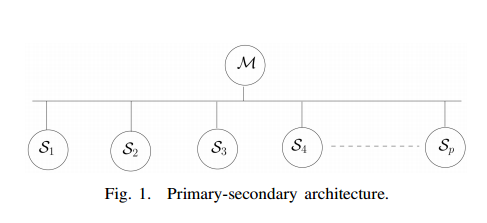
\includegraphics[scale=0.8]{primary_secondary.png}
\caption{}
\label{}
\end{figure}


The actual latency
and transmission times are dependent upon the
specific computer system. Although the processors
are inter-connected via the bus architecture, the
processors themselves and the inter-processor
communication among them may be heterogeneous.
The communication speed depends not only on the
interconnection architecture, but also on the power
of the processors as well.

为了最大化的利用带宽和处理器,提出了一种优化资源分配方式


In order to make the best use of available
communication bandwidth and processor power,
optimal resource allocation has to be carried out
in an efficient manner

挑战是选择处理器个数和寻找粒子数量映射到选择的处理器上


 In the multitarget particle
filter, the data transferred between the primary
and the secondary nodes vary according to the
number of targets. Therefore, the challenge here is
to select the number of processors and to find the
number of particles to be mapped onto the selected
processors.

为什么不固定一个很大的处理器单元个数。

As the number of targets increases,
the computational requirement for each particle
increases exponentially. This is due to the data
association taking place in each particle. Thus,
the optimal number of processors will be different
for a different number of targets. Because of the
communication overhead, using an unnecessarily
high number of processors will only degrade
performance

\textbf{Optimality Condition
}

主节点只和一个从节点交流,在每一个时刻


In the optimal scheduling, it is assumed that the
total work can be divided into finely decomposable
tasks (divisible load).
The communication mode
is exclusive and thus the primary processor can
communicate with only one secondary node at a
time
\begin{figure}[htp]
\centering
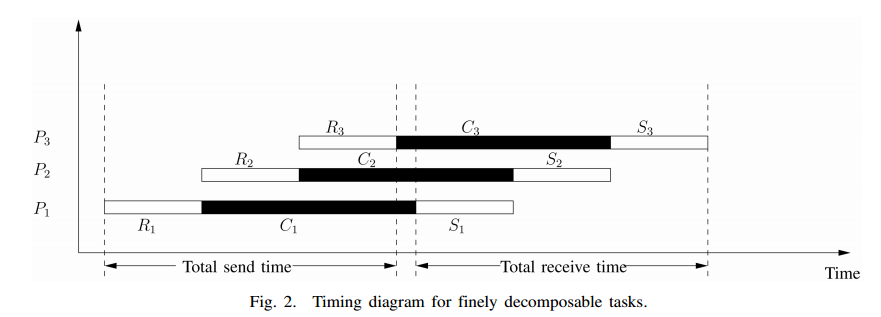
\includegraphics[scale=0.5]{timeing diagram.png}
\caption{}
\label{}
\end{figure}

\subsection{ SCHEDULING PROBLEM FORMULATION}

我们到假设是,处理器之间通过总线连接,同一时刻只有同一个交流。


 our assumption is that
the processors are connected via bus architecture,
where only one communication is allowed. Therefore,
the primary processor cannot start receiving data from a secondary processor even after the previous
secondary processor finishes computation because of
high communication load。

这种情况下,全部处理器用来计算并不是最优的。

Then one has to adopt an optimization
formulation to find the optimal number of processors
and the optimal number of particles to be mapped
among the selected processors.

\subsection{DRPF Algorithm}

\begin{figure}[htp]
\centering
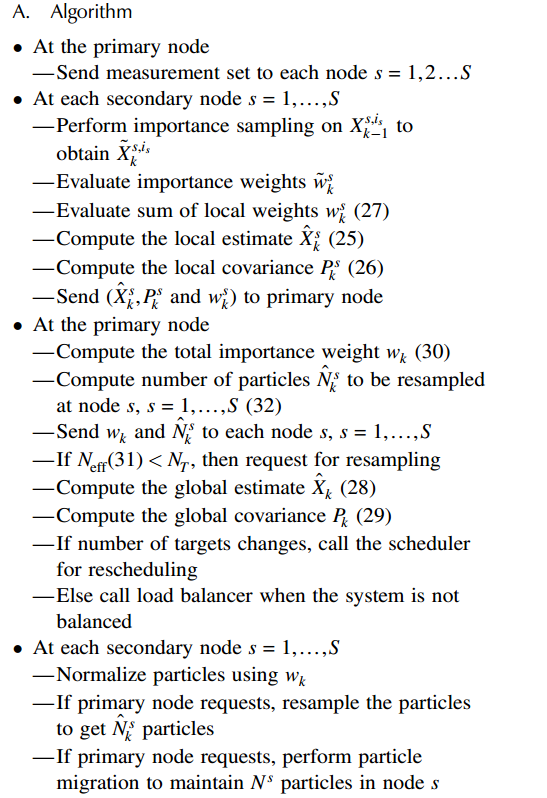
\includegraphics[scale=0.6]{Algorithm_parallel.png}
\caption{}
\label{}
 
\end{figure}
 
 
\subsection{Load Balancing}

load imbalance factor $\Phi(k) $   is used in the profitability(收益性;盈利能力)
determination process

The load balancing factor
is weighted against load balancing overhead to
determine whether the load balancing should be
performed or not


\end{CJK}
\end{document}